%%%%%%%%%%%%%%%%%%%%%%%%%%%%%%%%%%%%%%%%%%%%%%%%%%%%%%%%%%%%%%%%%%%%%%%%%%%%%%%%
%%%%%%%%%%%%%%%%%%   Vorlage für eine Abschlussarbeit   %%%%%%%%%%%%%%%%%%%%%%%%
%%%%%%%%%%%%%%%%%%%%%%%%%%%%%%%%%%%%%%%%%%%%%%%%%%%%%%%%%%%%%%%%%%%%%%%%%%%%%%%%

% Erstellt von Maximilian Nöthe, <maximilian.noethe@tu-dortmund.de>
% ausgelegt für lualatex und Biblatex mit biber

% Kompilieren mit 
% lualatex dateiname.tex
% biber dateiname.bcf
% lualatex dateiname.tex
% lualatex dateiname.tex




%------------------------------------------------------------------------------
%---------------- Docmentenklasse, Layout und Ränder: -------------------------
%------------------------------------------------------------------------------

\documentclass[
        paper=a4,               % Papierformat DIN A4
        BCOR=12mm,              % 12mm Binderandkorrektur
        parskip=half,           % Absätze als halbe Leerzeile
        cleardoublepage=plain,  % Keine Kopf/Fußzeile auf Leerseiten
        bibliography=totoc,     % Bibliographie als nicht-nummeriertes 
                                % Kapitel im Inhaltsverzeichnis
        %open=right,             % Kapitel beginnen immer aufrechten Seiten
        open=any,               % Kapitel dürfen auf beiden Seiten beginnen
        captions=tableheading,  % Spacing für Captions über Tabellen an
        headsepline,            % Linie unter der Kopfzeile
        titlepage=firstiscover, % Titelseite ist Deckblatt, symmetrische Ränder
        numbers=noenddot,       % keine Punkte nach Abilldungs/Kapitel/Tabellen Nummerierung
        headings=normal         % kleinere Überschriften
    ]
    {scrbook}


% Beschränkung auf chapter und section im Inhaltsverzeichnis:            
\setcounter{tocdepth}{1}


%------------------------------------------------------------------------------
%----------------------------- Encoding: --------------------------------------
%------------------------------------------------------------------------------

% falls es Probleme mit Umlauten oder Symbolen gibt, überprüfen ob die Texfiles 
% utf8-codiert sind, evtl auch wieder einkommentieren
%\usepackage[utf8]{luainputenc}

%------------------------------------------------------------------------------
%------------------------------ Sprache und Schrift: --------------------------
%------------------------------------------------------------------------------

% \usepackage[ngerman]{babel}     % Deutsche Spracheinstellungen
\usepackage{polyglossia}
\setdefaultlanguage{german}

\usepackage{csquotes}           % stellt den \enquote{} Befehl


% Schriftarten einstellen, hier können auch Schriftarten des Systems genutzt werden:

%\usepackage[protrusion=true, expansion]{microtype}
\usepackage{fontspec}
\defaultfontfeatures{Ligatures=TeX}
\setmainfont{Latin Modern Roman}
\setsansfont{Latin Modern Sans}
\setmonofont{Latin Modern Mono}



%------------------------------------------------------------------------------
%-------------------------Pakete für Kopf/Fußzeile: ---------------------------
%------------------------------------------------------------------------------

%\usepackage{scrpage2}
%\pagestyle{scrheadings}


%------------------------------------------------------------------------------
%------------------------ Für die Matheumgebung--------------------------------
%------------------------------------------------------------------------------

\usepackage{amsmath}
\usepackage{amssymb}
\usepackage{mathtools}
\usepackage{unicode-math}
\setmathfont{Latin Modern Math}

\usepackage{xfrac}  % schöne Brüche im Text mit \sfrac{}{}


%Gleichungsnummern Kapitel.Unterkapitel.Gleichung
\renewcommand{\theequation}{\thesection{}.\arabic{equation}}
\numberwithin{equation}{chapter}
\numberwithin{equation}{section}

%------------------------------------------------------------------------------
%---------------------------- Einheiten ---------------------------------------
%------------------------------------------------------------------------------

\usepackage[locale=DE, separate-uncertainty=true, per-mode=fraction]{siunitx}
\sisetup{math-micro=\text{µ},text-micro=µ}

%------------------------------------------------------------------------------
%------------------------------ Tabellen: -------------------------------------
%------------------------------------------------------------------------------

\usepackage{tabulary}
\usepackage{booktabs}       % stellt \toprule, \midrule, \bottomrule
\usepackage{threeparttable} % für komplexere Tabellen

%------------------------------------------------------------------------------
%------------------------------ Grafiken: -------------------------------------
%------------------------------------------------------------------------------

\usepackage[]{graphicx}         % einbinden von Grafiken
\usepackage{captcont}           % Für Tabellen oder Abbildungen über mehrere Seiten
\usepackage[
            labelfont=bf,       % "Abbildung 1" bzw. "Tabelle 1" fett
            width=0.9\textwidth,
            format=plain
           ]{caption}

\usepackage{subcaption}   % for subfigures


%------------------------------------------------------------------------------
%------------------------------ Bibliographie ---------------------------------
%------------------------------------------------------------------------------

\usepackage[backend=biber]{biblatex}    % Biblatex mit biber
    \addbibresource{references.bib}     % die Bibliographie einbinden

\DefineBibliographyStrings{ngerman}{andothers = {{et\,al\adddot}}}


%------------------------------------------------------------------------------
%------------------------------ Sonstiges: ------------------------------------
%------------------------------------------------------------------------------


\usepackage[pdfusetitle,unicode]{hyperref}
\usepackage{xcolor}
\usepackage{eurosym}
\usepackage[ngerman]{varioref}


%------------------------------------------------------------------------------
%-------------------------    Angaben zur Arbeit   ----------------------------
%------------------------------------------------------------------------------

%Titel der Arbeit
\newcommand{\thetitle}{\LaTeX-Vorlage für die Bachelorarbeit}
\newcommand{\Jahr}{2014}
\newcommand{\Geburtsort}{Castrop-Rauxel}
\newcommand{\Lehrstuhl}{Experimentelle Physik V}
\newcommand{\Betreuer}{Prof. Dr. Erstgutachter}
\newcommand{\Zweitgutachter}{Prof. Dr. Zweitgutachter}
\newcommand{\Abgabedatum}{11. Juli 2014}

%Author und Email-Adresse
\author{
    Maximilian Nöthe\\
    geboren in \Geburtsort
}

\title{\thetitle}
\date{\Jahr}

\subject{Arbeit zur Erlangung des akademischen Grades\\Bachelor of Science}
\publishers{Lehrstuhl für \Lehrstuhl \\ Fakultät Physik \\ Technische Universität Dortmund}

%Gutachterseite
\lowertitleback{
    \begin{tabbing}
        Erstgutachter: \hspace{3em}\=   \Betreuer \\ 
        Zweitgutachter: \> \Zweitgutachter\\
        Abgabedatum: \>\Abgabedatum
    \end{tabbing}
}




\begin{document}
\frontmatter
\maketitle
% hier beginnt der Vorspann, nummeriert in römischen Zahlen
\thispagestyle{plain}
\section*{Kurzfassung}

\textbf{\large Empfohlen wird die Verwendung dieser Vorlage mit der jeweils aktuellsten TeXLive Version (Linux, Windows) bzw. MacTeX Version (MacOS).
Aktuell ist dies TeXLive 2014. Download hier: 
Wichtig ist auch, dass die Source-Dateien UTF-8 kodiert sind. Dies
ist nur unter Windows ein Problem, benutzen Sie einen Editor, der
utf-8 unterstützt (z.B. TexMaker ab V4, notepad++, sublime).
}

\href{https://www.tug.org/texlive/}{\textbf{\large https://www.tug.org/texlive/}}

Eine aktuelle Version dieser Vorlage gibt es unter 

\href{https://github.com/MaxNoe/VorlageBachelorArbeit}{www.github.com/MaxNoe/VorlageBachelorArbeit}.

Eine Variante, in der bestimmte Elemente in TU-Farben gehalten sind, steht unter 

\href{https://github.com/MaxNoe/VorlageBachelorArbeit/tree/tu-farben}{www.github.com/MaxNoe/VorlageBachelorArbeit/tree/tu-farben}  

zur Verfügung.

Falls es Probleme mit der Vorlage gibt, einfach ein \emph{Issue} auf GitHub aufmachen oder eine Email an
\href{mailto:maximilian.noethe@tu-dortmund.de}{maximilian.noethe@tu-dortmund.de} schreiben.


Hier steht eine Kurzfassung der Arbeit in deutscher Sprache inklusive der Zusammenfassung der
Ergebnisse.
Zusammen mit der englischen Zusammenfassung muss sie auf diese Seite passen.

\section*{Abstract}

The abstract is a short summary of the thesis in English, together with the German summary it has to fit on this page.

\tableofcontents

\mainmatter
% Hier beginnt der Inhalt mit Seite 1 in arabischen Ziffern
\chapter{Einleitung}
Hier Erfolgt eine kurze Einleitung in die Thematik der Bachelorarbeit.
Die Einleitung muss kurz sein, damit die vorgegebene Gesamtlänge der 
Arbeit, exklusive Anhang von 25 Seiten nicht überschritten wird. 
Die Beschränkung der Seitenzahl sollte man ernst nehmen,
da Überschreitung zu Abzügen in der Note führen kann. 
Um der Längenbeschränkung zu genügen, darf auch nicht an der Schriftgröße,
dem Zeilenabstand oder dem Satzspiegel (bedruckte Fläche der Seite) manipuliert werden.

\chapter{Struktur der Arbeit}

Eine mögliche Struktur der Arbeit sieht wie folgt aus:

\begin{enumerate}
    \item \textbf{Einleitung}\\
        In der \emph{kurzen} Einleitung wird die Motivation für die Arbeit
        dargestellt und ein Einblick in die kommenden Kapitel gegeben.
    \item \textbf{Theoretische Grundlagen}\\
        Alles was an theoretischen Grundlagen benötigt wird, sollte auch eher kurz gehalten werden.
        Statt Grundlagenwissen zu präsentieren, eher auf die entsprechenden Lehrbücher verweisen.
        Etwa: Tiefer gehende Informationen zur klassischen Mechanik entnehmen Sie bitte \cite{kuypers}.
    \item \textbf{Ergebnisse} \\
        Der eigentliche Teil der Arbeit, das was getan wurde.
    \item \textbf{Zusammenfassung und Ausblick} \\
        Zusammenfassung der Ergebnisse, Optimierungsmöglichkeiten, mögliche weitergehende Untersuchungen.
\end{enumerate}

Die Gliederung sollte auf der einen Seite nicht zu fein sein, auf der anderen Seite
sollten sich klar unterscheidende Abschnitte auch kenntlich gemacht werden.

In der hier verwendeten \KOMAScript-Klasse \texttt{scrbook} ist die oberste Gliederungsebene,
die in der Bachelorarbeit verwendet werden sollte, das \texttt{\textbackslash chapter}.

Ein Kapitel sollte erst dann in tiefere Gliederungsebenen unterteilt werden, wenn es auch wirklich etwas zu unterteilen gibt. Es sollte keine Kapitel mit nur einem Unterkapitel (\texttt{\textbackslash section}) geben.

In dieser Vorlage ist die Tiefe des Inhaltsverzeichnisses auf \texttt{chapter} und \texttt{section} beschränkt. Möchten Sie diese Beschränkung aufheben, entfernen Sie den Befehl
\begin{verbatim}
            \setcounter{tocdepth}{1}
\end{verbatim}
aus der Präambel oder ändern Sie den Zahlenwert entsprechend. Das Inhaltsverzeichnis sollte für eine Bachelorarbeit auf eine Seite passen.

\chapter{Wichtige Hinweise zum Dokument}\label{make}

Diese Vorlage ist auf die Kompilierung mit \texttt{lualatex} ausgelegt. 
Als Dokumentenklasse  wird die \KOMAScript\-Klasse \texttt{scrbook} verwendet.
Falls Sie Änderungen am Layout vornehmen möchten, lesen Sie die \KOMAScript-Dokumentation: \cite{koma}.

Lesenswert ist außerdem das \LaTeX-Tabu: \cite{l2tabu}, sowie \emph{Modern Packages for \LaTeX} von Philipp Leser: \cite{pleser}.

\section{Erstellen des Ausgabedokuments mit Make}

Für diese Vorlage wird ein Makefile zur Verfügung gestellt, welches automatisch alle Schritte ausführt, die für das fertige Dokument nötig sind. Make prüft, ob die Quelldateien verändert wurden, falls nicht, werden auch keine Befehle ausgeführt.

Folgende Befehle werden durch das Makefile druchgeführt, falls sich die Quelldateien verändert haben:

\begin{enumerate}
    \item \texttt{lualatex BachelorArbeit.tex}
    \item \texttt{biber BachelorArbeit.tex}
    \item \texttt{lualatex BachelorArbeit.tex}
    \item \texttt{lualatex BachelorArbeit.tex}
    \item verschieben der Hilfs- und Logdateien in den Ordner logfiles
\end{enumerate}


Download und weitere Informationen zu Make gibt es unter \cite{make}.
Wenn Sie Make installiert haben, rufen Sie einfach in der Konsole im Verzeichnis der Arbeit den Befehl \texttt{make}.

\section{Erstellen des Ausgabedokuments mit Texmaker}

Ein beliebter Editor für alle Betriebssysteme ist Texmaker, Download unter \cite{texmaker}.
Damit Texmaker das Dokument korrekt kompiliert, fügen sie einen benutzerdefinierten Befehl hinzu:
\begin{enumerate}
    \item Klicken sie oben in der Menüleiste auf \emph{Benutzer/in}
    \item Klick auf \emph{Eigene Befehle}
    \item Klich auf \emph{Eigene Befehle editieren}, dort können Sie bis zu 5 eigene Befehle definieren
    \item Geben Sie dem Befehl unter \emph{Menüeintrag} einen Namen und tragen sie folgende Zeile in das Befehlsfeld ein: \\
        \texttt{lualatex \%.tex | biber \%.bcf | lualatex \%.tex | lualatex \%.tex}
    \item Bestätigen Sie mit \emph{OK}
\end{enumerate}

\begin{figure}[!h]
    \centering
    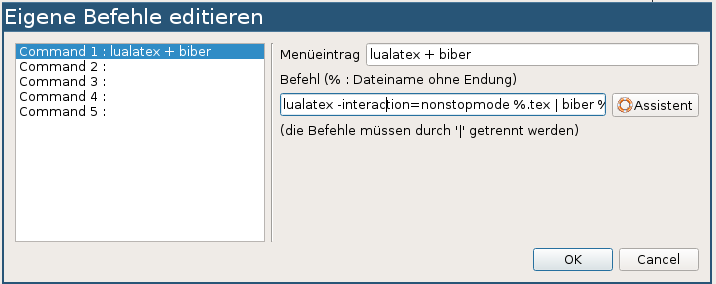
\includegraphics[width=12cm]{Plots/texmaker.png}
    \caption{Screenshot zur Erstellung des Kompilier-Befehls in Texmaker}
    \label{fig:texmaker}
\end{figure}


In Abbildung \ref{fig:texmaker} ist ein Screenshot des Befehlsmenü gezeigt. Ihren Befehl können Sie nun im Drop-Down-Menü zum 
kompilieren des Dokuments auswählen und mit einem Klick auf den Pfeil starten.


\chapter{\LaTeX-Grundlagen}

Bitte beachten Sie beim Schreiben der Arbeit folgende Konventionen bzw. Grundlagen:

\begin{itemize}
    \item \textbf{Abschnitte und Zeilenumbrüche} \\
        Es sollten im Fließtext keine Zeilenumbrüche mit \textbackslash\textbackslash \ erzwungen werden.
        Schreiben Sie höchsten einen Satz in eine Code-Zeile.
        Absätze werden im Code mit einer Leerzeile markiert und dann entsprechend der Einstellung von \texttt{parskip} in der Dokumentenklasse gesetzt.
    \item \textbf{Kursiv/Aufrecht} \\
        \begin{itemize}
            \item Variablen und physikalische Größen werden kursiv gesetzt. 
            \item Einheiten werden immer aufrecht und mit einem halben Leerzeichen Abstand zur Zahl gesetzt. Nutzen Sie \texttt{siunitx}!
            \item Mathematische Konstanten und Funktionenwerden ebenfalls aufrecht gesetzt. Zum Beispiel de Eulersche Zahl e, das imaginäre i und das infinitesimale d.
                Im Mathematikmodus können Sie dies mit dem Befehl \verb_\mathrm{}_ erreichen. Für die Funktionen stell \LaTeX \ Befehle bereit, z.B. \verb+\arccos+.
            \item Integrand und ein $\mathrm{d}x$ sollten ebenfalls durch ein kleines Leerzeichen (\verb+\,+) getrennt werden.
        \end{itemize}
        


\end{itemize}

\section{Zahlen und Einheiten}

Jede Zahl, jede Einheit und jede Zahl mit Einheit sollte mit Hilfe der in dem Paket \texttt{siunitx} zur Verfügung gestellten Befehle gesetzt werden.
Grundsätzlich gilt: Einheiten werden aufrecht gesetzt und haben ein kleines Leerzeichen (\verb+\,+) Abstand zu ihrer Zahl. 
Werden Fließkommazahlen ohne \texttt{siunitx} gesetzt, entsteht ein hässlicher Leerraum zwischen Komma und erster Nachkommastelle, da \LaTeX \ das Komma nicht als Dezimaltrennzeichen, sondern als Satzzeichen interpretiert.

Das Paket wurde mit deutschen Spracheinstellungen (also mit Komma als Dezimaltrennzeichen und $\cdot$ zwischen Zahl und Zehnerpotenz) geladen, sowie mit den Einstellungen, dass die Standardabweichung stets durch $\pm$ abgetrennt wird und Einheiten falls nötig als Brüche ausgegeben werden.

\begin{table}[!h]
    \centering
    \caption{Beispiele für siunitx}
    \label{tab:si}
    \begin{tabular}{l r}
        \toprule
        Befehl     &   Ergebnis \\
        \midrule
        \verb+\num{1.2345}+ & \num{1.2345} \\
        \verb+\num{1.2e3}+ & \num{1.2e3} \\
        \verb_\num{1.2 +- 0.2}_ & \num{1.2+-0.2} \\
        \verb+\num{10000}+ & \num{10000} \\
        \verb+\si{\meter\per\second}+ & \si{\meter\per\second} \\
        \verb+\SI{1.2(1)}{\micro\ampere}+ & \SI{1.2(1)}{\micro\ampere} \\
        \verb+\SI{1.2\pm0.1e3}{\kilo\gram\per\cubic\meter}+ & \SI{1.2\pm0.1e3}{\kilo\gram\per\cubic\meter} \\
        \bottomrule 
    \end{tabular}
\end{table}

Das Paket stellt unter anderem die drei wichtigen Befehle
\begin{itemize}
    \item \texttt{\textbackslash num\{Zahl\}},
    \item \texttt{\textbackslash si\{Einheit\}} und
    \item \texttt{\textbackslash SI\{Zahl\}\{Einheit\}}
\end{itemize}
zur Verfügung.
Diese Befehle sollten stets genutzt werden, wenn Zahlen angegeben werden. 
Sie funktionieren sowohl im Text- als auch im Mathematikmodus.
In Tabelle \ref{tab:si} sind einige Beispiele aufgetragen. Bitte lesen Sie die Dokumentation \cite{siunitx}.

\section{Das Literaturverzeichnis}

Das Literaturverzeichnis wird mit Hilfe von BibLaTeX und biber erstellt.
Tragen Sie alle ihre Quellen in die Datei \texttt{references.bib} ein, Sie enthält bereits
einige Beispiele. Für weitere Informationen lesen Sie bitte die Dokumentation \cite{biblatex}.

Im Text können Sie mit \verb_\cite{kürzel}_ zitieren. Seitenzahlen geben Sie in eckigen Klammern an:
\verb_\cite[S.~10]{kürzel}_. Das Literaturverzeichnis ist so eingestellt, dass es Ihre Quellen in alphabetischer Reihenfolge nummeriert.

Damit das Literaturverzeichnis erstellt wird, ist ein Aufruf von \texttt{biber} nach einem ersten kompilieren mit \texttt{lualatex} nötig.
Danach muss das Dokument erneut mit \texttt{lualatex} kompiliert werden. 

Zum korrekten Kompilieren des Dokuments siehe Kapitel \ref{make}.

\chapter{Abbildungen und Tabellen}

\section{Abbildungen}

Achten Sie bei ihren Plots auf ausreichend große Achsenbschriftungen, ausreichende Schriftdicken und gut unterscheidbare Farben.
Im Idealfall haben Sie im Plot und der Arbeit die gleiche Schriftgröße und Schriftart.
Dies lässt sich durch Erstellen des Plots in der korrekten Größe und einbinden mit dem optionalen Argument \texttt{scale=1} erreichen. Ein Beispiel sehen Sie in Abbildung \ref{fig:bsp}.

Nutzen Sie wenn möglich Vektorgrafiken (pdf) und nur in Ausnahmen Rastergrafiken wie .png oder .jpg.
Setzen Sie Punkte hinter Abbildungsunterschriften.

\begin{figure}
    \centering
    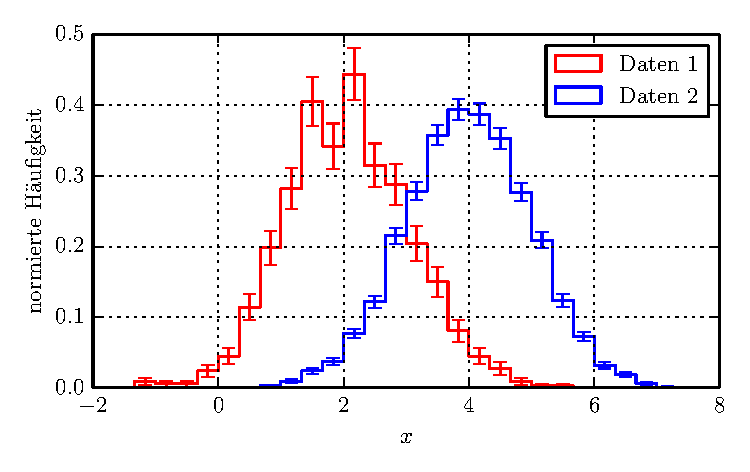
\includegraphics[scale=1]{./Plots/Histogramm.pdf}
    \caption{Ein Histogramm mit Fehlerbalken für zwei Datensätze, Schriftgröße und -art entsprechen der des Dokuments.}
    \label{fig:bsp}
\end{figure}

\section{Tabellen}

Tabellen sollten so einfach wie möglich aufgebaut sein, verzichten Sie auf zu viele Linien. In fast allen Fällen reichen drei horizontale Linien aus, jeweils über und unter der Tabelle und zwischen den Spaltenüberschriften und der eigentlichen Tabelle.

Das Paket \texttt{booktabs} stellt hierfür die Befehle \verb_\toprule_, \verb_\midrule_ und 
\verb_\bottomrule_ zur Verfügung.
Das Paket \texttt{siunitx} stellt eine extrem mächtige neue Spalteneinstellung bereit: \texttt{S}, mit ihr können Zahlen und Einheiten sehr sauber und gut ausgerichtet gesetzt werden.

Diese Vorlage geht von Tabellenüberschriften aus, möchten Sie dagegen Tabellenunterschriften entfernen Sie das entsprechende optionale Argument für die Dokumentenklasse in der Präambel.

Eine Beispiel ist Tabelle \ref{tab:bsp}.

\begin{table}
    \centering
    \caption{Beispieltabelle mit willkürlichen Werten, für die Zahlenwerte wurde die S-Option aus SIunitx verwendet, für die Einheitenspalte die s-Option.}
    \label{tab:bsp}
    \begin{tabular}{l S[table-format=3.2] S[table-format=3.2(2)] s}
        \toprule
        Variable    & {Theoriewert} & {gemessener Wert} & {Einheit}\\
        \midrule
        Druck       & 1,23      & 1,31(5)   & \pascal \\
        Temperatur  & 273,15    & 273,5(2) & \kelvin \\
        \bottomrule
    \end{tabular}
\end{table}


\appendix
% Hier beginnt der Anhang, nummeriert in lateinischen Buchstaben
\chapter{Ein Anhangskapitel}

Hier könnte ein Anhang stehen.


\backmatter
\printbibliography

\cleardoublepage
\thispagestyle{empty}
\section*{Eidesstattliche Versicherung}
Ich versichere hiermit an Eides statt, dass ich die vorliegende Bachelorarbeit mit dem Titel \enquote{\thetitle} selbst\-ständig und ohne unzulässige fremde Hilfe erbracht habe.
Ich habe keine anderen als die angegebenen Quellen und Hilfsmittel benutzt, sowie wörtliche und sinngemäße Zitate kenntlich gemacht. 
Die Arbeit hat in gleicher oder ähnlicher Form noch keiner Prüfungsbehörde vorgelegen.

\vspace*{1cm}\noindent
\begin{tabular}{@{}p{0.4\textwidth}@{\hspace{0.2\textwidth}}p{0.4\textwidth}@{}}
\rule{\linewidth}{0.25pt}& \rule{\linewidth}{0.25pt}\\
Ort, Datum & Unterschrift
\end{tabular}

\subsection*{Belehrung}
Wer vorsätzlich gegen eine die Täuschung über Prüfungsleistungen betreffende Regelung einer Hochschulprüfungsordnung verstößt, handelt ordnungswidrig.
Die Ordnungswidrigkeit kann mit einer Geldbuße von bis zu \SI[round-mode=places, round-precision=2]{50000}{€} geahndet werden. 
Zuständige Verwaltungsbehörde für die Verfolgung und Ahndung von Ordnungswidrigkeiten ist der Kanzler/die Kanzlerin der Technischen Universität Dortmund. 
Im Falle eines mehrfachen oder sonstigen schwerwiegenden Täuschungsversuches kann der Prüfling zudem exmatrikuliert werden \mbox{(\S63 Abs. 5 Hochschulgesetz --HG--).}

Die Abgabe einer falschen Versicherung an Eides statt wird mit Freiheitsstrafe bis zu 3 Jahren oder mit Geldstrafe bestraft.

Die Technische Universität Dortmund wird ggf.\ elektronische Vergleichswerkzeuge (wie z.\,B.\ die Software \enquote{turnitin}) zur Überprüfung von Ordnungswidrigkeiten in Prüfungsverfahren nutzen. \\[\baselineskip]

\noindent Die oben stehende Belehrung habe ich zur Kenntnis genommen.\\[1cm]
\begin{tabular}{@{}p{0.4\textwidth}@{\hspace{0.2\textwidth}}p{0.4\textwidth}@{}}
\rule{\linewidth}{0.25pt}& \rule{\linewidth}{0.25pt}\\
Ort, Datum & Unterschrift
\end{tabular}


\end{document}
